\chapter{Darknet移植}
\section{Darknet介绍\cite{darknet13}}
Darknet是一个开源的C语言神经网络框架,由著名的机器视觉专家Joseph Redmon开发。Darknet性能优异,安装简单,在目标识别领域有广泛应用的YOLO模型\cite{yolov3}的最初版本就是在这个框架下开发的。作为作为“神威 · 太湖之光”并行编程的入门练习,Darknet有如下优点\cite{darknet_note}:
\begin{itemize}
    \item 易于安装:在makefile里面选择自己需要的附加项(cuda,cudnn,opencv等)直接make即可;
    \item 没有任何依赖项:整个框架都用C语言进行编写,可以不依赖任何库,连opencv作者都编写了可以对其进行替代的函数;
    \item 结构清晰:其框架的基础文件都在src文件夹,而定义的一些检测、分类函数则在example文件夹,可根据需要直接对源代码进行查看和修改;
    \item 友好python接口:虽然darknet使用c语言进行编写,但是也提供了python的接口,通过python函数,能够使用python直接对训练好的.weight格式的模型进行调用;
    \item 易于移植:该框架部署十分简单,且可以根据机器情况,使用cpu和gpu,特别是检测识别任务的本地端部署,darknet会显得异常方便。
\end{itemize}

此外,由于Darknet是一个神经网络框架,其中的主要运算任务都可以以矩阵计算的形式所表述,这使得Darknet的移植和优化有助于读者对矩阵和并行更加深入的理解。最后,Darknet框架整体结构比较成熟完整,读者能在移植和优化过程中了解到优秀的机器学习框架的架构与编写方式,对软件架构能力的提升有一定帮助。

\section{Darknet源码结构}
从Joseph Redmon的个人网站或Github上下载得到的Darknet源码包解压后可得到如图所示的文件和文件夹,各文件和文件夹的作用如下\cite{darknet_note}:
\begin{itemize}
    \item cfg文件夹内是一些模型的架构,每个cfg文件类似于caffe的prototxt文件,通过该文件定义的整个模型的架构;
    \item data文件夹内放置了一些label文件,如coco9k的类别名等,和一些样例图,主要在训练和测试时使用;
    \item src文件夹内是最底层的框架定义文件,所有层的定义等最基本的函数全部在该文件夹内,是Darknet框架的源码所在;
    \item examples文件夹是更为高层的一些函数,如检测函数,识别函数等,这些函数直接调用了底层的函数,是对底层函数的封装;
    \item include文件夹,顾名思义,存放头文件的地方;
    \item python文件夹里是使用python对模型的调用方法,基本都在darknet.py中。要实现python的调用,还需要用到darknet的动态库libdarknet.so;
    \item scripts文件夹中是一些脚本,如下载coco数据集,将voc格式的数据集转换为训练所需格式的脚本等;
    \item 一系列和功能无关的license文件;
    \item 本章的重点Makefile文件,用于框架的编译和运行。
\end{itemize}

\section{Darknet的移植}
\subsection{Linux make和Makefile介绍其二}
在\ref{subsec:Makefile介绍}节中已经介绍过Makefile的文件结构和Linux make的基本使用方法,在本节中将进一步介绍Makefile文件中的变量定义和计算,为理解Darknet的编译过程打下基础。

在Makefile文件中,如果有某些指令和名称比较长或是需要在文件不同位置多次使用,为了保证可读性和修改的方便则需要用类似C语言宏定义的方式,用一些“宏”(更准确地说应该是变量)代表这些指令或名称。Linux make和Makefile即提供了这样的功能,这种功能的存在也使得Makefile被称为“make脚本”\footnote{为啥叫“脚本”?“脚本”的英文是“script”,可以联想两种解释型编程语言:js和python。js全称是“JavaScript”,python的源代码文件也叫“python script”,它们都是以解释器解释脚本文件中源代码的方式运行的。make也可以看作是一个解释型编程语言的解释器,Makefile就是它读入并解释的脚本文件,\ref{subsec:Makefile介绍}节和本节就是在介绍这个编程语言的语法}。这一功能可以概况为如下几种语法:
\begin{itemize}
    \item 变量定义:
    \begin{lstlisting}
[变量名]=[值];
    \end{lstlisting}
    \item 变量调用:
    \begin{lstlisting}
$([变量名])
    \end{lstlisting}
    \item 变量修改:
    \begin{lstlisting}
[变量名]+=$([变量名])或[值]
    \end{lstlisting}
    \begin{lstlisting}
[变量名]=$([变量名])或[值]+$([变量名])或[值]+...
    \end{lstlisting}
    \item 变量比较和if语句:
    \begin{lstlisting}
ifeq ($([变量名]), $([变量名])或[值])
一些操作
endif
    \end{lstlisting}
\end{itemize}

Makefile中的所有变量均是字符串,变量修改中的“+”表示的就是字符串的连接,变量比较就是字符串的比较;字符串的调用可以在文件的任何地方,Linux make在运行时会自动将Makefile中的变量调用替换为变量对应的字符串\footnote{就像C语言的宏一样}。例如\ref{subsec:编写Makefile}中的Makefile:
\begin{lstlisting}
arrAdd:master_arrAdd.o slave_arrAdd.o
    sw5cc -hybrid master_arrAdd.o slave_arrAdd.o -o arrAdd
master_arrAdd.o:master_arrAdd.c
    sw5cc -host -c master_arrAdd.c
slave_arrAdd.o:slave_arrAdd.c
    sw5cc -slave -c slave_arrAdd.c
clean:
    rm master_arrAdd.o slave_arrAdd.o arrAdd
run:arrAdd
    bsub -I -b -q q_sw_expr -n 1 -cgsp 64 ./arrAdd
\end{lstlisting}
把其中的输出文件名“arrAdd”、两个.o文件和bsub的运行选项用变量表示,可将Makefile改写如下:
\begin{lstlisting}
OUTPUT=arrAdd
OFILES=master_arrAdd.o slave_arrAdd.o
OPT=-I -b
OPT+=-q q_sw_expr
OPT+=-n 1
OPT+=-cgsp 64
$(OUTPUT):$(OFILES)
    sw5cc -hybrid $(OFILES) -o $(OUTPUT)
master_arrAdd.o:master_arrAdd.c
    sw5cc -host -c master_arrAdd.c
slave_arrAdd.o:slave_arrAdd.c
    sw5cc -slave -c slave_arrAdd.c
clean:
    rm $(OFILES) $(OUTPUT)
run:$(OUTPUT)
    bsub $(OPT) ./$(OUTPUT)
\end{lstlisting}

\subsection{Darknet的Makefile}
官网下载的Darknet源码中的Makefile文件如附录\ref{apdx:Darknet的Makefile}所示,本节将对这个Makefile文件及其所定义的编译过程进行解析。

\subsection{数学公式}

比如Navier-Stokes方程(方程~\eqref{eq:ns}):
\begin{equation} \label{eq:ns}
    \adddotsbeforeeqnnum%
    \begin{cases}
        \frac{\partial \rho}{\partial t} + \nabla\cdot(\rho\Vector{V}) = 0 \ \mathrm{times\ math\ test: 1,2,3,4,5}, 1,2,3,4,5\\
        \frac{\partial (\rho\Vector{V})}{\partial t} + \nabla\cdot(\rho\Vector{V}\Vector{V}) = \nabla\cdot\Tensor{\sigma} \ \text{times text test: 1,2,3,4,5}\\
        \frac{\partial (\rho E)}{\partial t} + \nabla\cdot(\rho E\Vector{V}) = \nabla\cdot(k\nabla T) + \nabla\cdot(\Tensor{\sigma}\cdot\Vector{V})
    \end{cases}
\end{equation}
\begin{equation}
    \adddotsbeforeeqnnum%
    \frac{\partial }{\partial t}\int\limits_{\Omega} u \, \mathrm{d}\Omega + \int\limits_{S} \unitVector{n}\cdot(u\Vector{V}) \, \mathrm{d}S = \dot{\phi}
\end{equation}
\[
    \begin{split}
        \mathcal{L} \{f\}(s) &= \int _{0^{-}}^{\infty} f(t) e^{-st} \, \mathrm{d}t, \ 
        \mathscr{L} \{f\}(s) = \int _{0^{-}}^{\infty} f(t) e^{-st} \, \mathrm{d}t\\
        \mathcal{F} {\bigl (} f(x+x_{0}) {\bigr )} &= \mathcal{F} {\bigl (} f(x) {\bigr )} e^{2\pi i\xi x_{0}}, \ 
        \mathscr{F} {\bigl (} f(x+x_{0}) {\bigr )} = \mathscr{F} {\bigl (} f(x) {\bigr )} e^{2\pi i\xi x_{0}}
    \end{split}
\]

数学公式常用命令请见 \href{https://en.wikibooks.org/wiki/LaTeX/Mathematics}{WiKibook Mathematics}。artracom.sty中对一些常用数据类型如矢量矩阵等进行了封装,这样的好处是如有一天需要修改矢量的显示形式,只需单独修改artracom.sty中的矢量定义即可实现全文档的修改。

\subsection{数学环境}

\begin{axiom}
   这是一个公理。 
\end{axiom}
\begin{theorem}
   这是一个定理。 
\end{theorem}
\begin{lemma}
   这是一个引理。 
\end{lemma}
\begin{corollary}
   这是一个推论。 
\end{corollary}
\begin{assertion}
   这是一个断言。 
\end{assertion}
\begin{proposition}
   这是一个命题。 
\end{proposition}
\begin{proof}
    这是一个证明。
\end{proof}
\begin{definition}
    这是一个定义。
\end{definition}
\begin{example}
    这是一个例子。
\end{example}
\begin{remark}
    这是一个注。
\end{remark}

\subsection{表格}

请见表~\ref{tab:sample}。
\begin{table}[!htbp]
    \bicaption{这是一个样表。}{This is a sample table.}
    \label{tab:sample}
    \centering
    \footnotesize% fontsize
    \setlength{\tabcolsep}{4pt}% column separation
    \renewcommand{\arraystretch}{1.2}%row space 
    \begin{tabular}{lcccccccc}
        \hline
        行号 & \multicolumn{8}{c}{跨多列的标题}\\
        %\cline{2-9}% partial hline from column i to column j
        \hline
        Row 1 & $1$ & $2$ & $3$ & $4$ & $5$ & $6$ & $7$ & $8$\\
        Row 2 & $1$ & $2$ & $3$ & $4$ & $5$ & $6$ & $7$ & $8$\\
        Row 3 & $1$ & $2$ & $3$ & $4$ & $5$ & $6$ & $7$ & $8$\\
        Row 4 & $1$ & $2$ & $3$ & $4$ & $5$ & $6$ & $7$ & $8$\\
        \hline
    \end{tabular}
\end{table}

制图制表的更多范例,请见 \href{https://github.com/mohuangrui/ucasthesis/wiki}{ucasthesis 知识小站} 和 \href{https://en.wikibooks.org/wiki/LaTeX/Tables}{WiKibook Tables}。

\subsection{图片插入}

论文中图片的插入通常分为单图和多图,下面分别加以介绍:

单图插入:假设插入名为\verb|tc_q_criteria|(后缀可以为.jpg、.png、.pdf,下同)的图片,其效果如图\ref{fig:tc_q_criteria}。
\begin{figure}[!htbp]
    \centering
    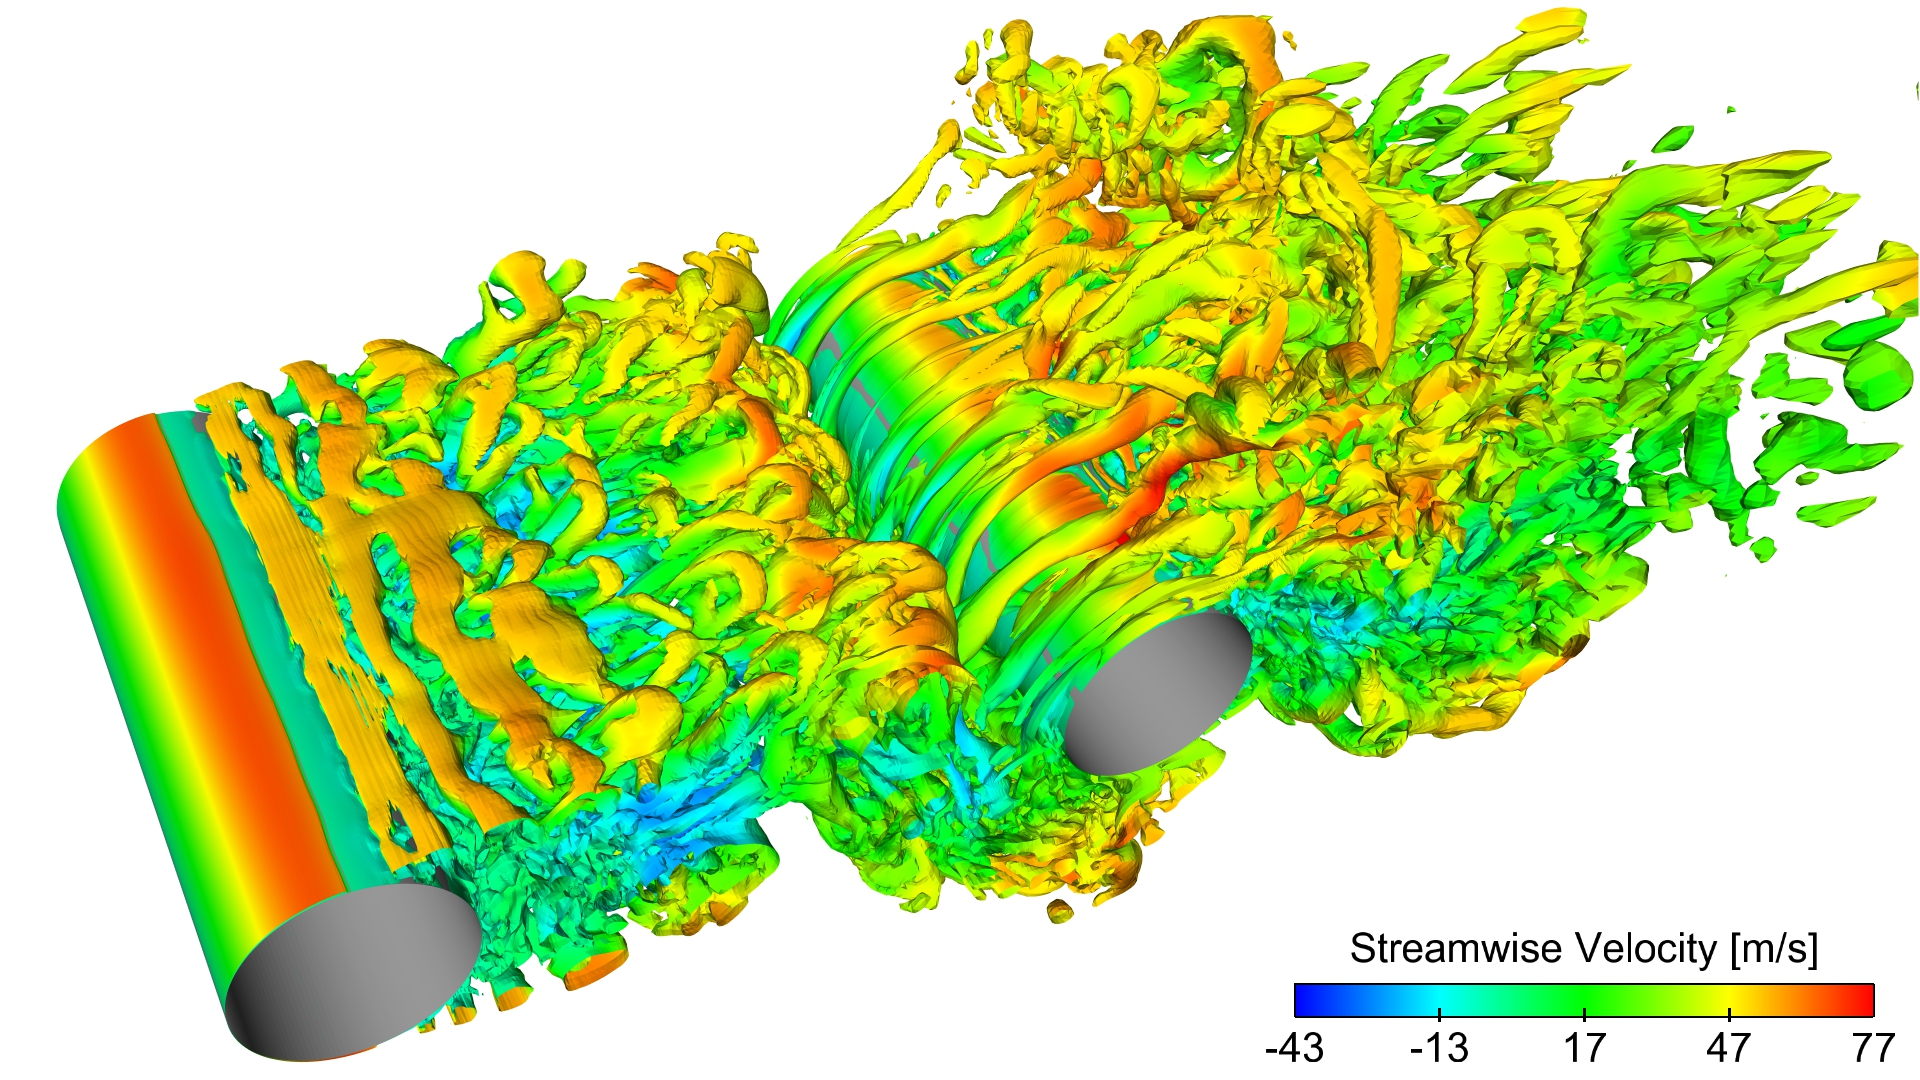
\includegraphics[width=0.40\textwidth]{tc_q_criteria}
    \bicaption{Q判据等值面图,同时测试一下一个很长的标题,比如这真的是一个很长很长很长很长很长很长很长很长的标题。}{Isocontour of Q criteria, at the same time, this is to test a long title, for instance, this is a really very long very long very long very long very long title.}
    \label{fig:tc_q_criteria}
\end{figure}

如果插图的空白区域过大,以图片\verb|shock_cyn|为例,自动裁剪如图\ref{fig:shock_cyn}。
\begin{figure}[!htbp]
    \centering
    %trim option's parameter order: left bottom right top
    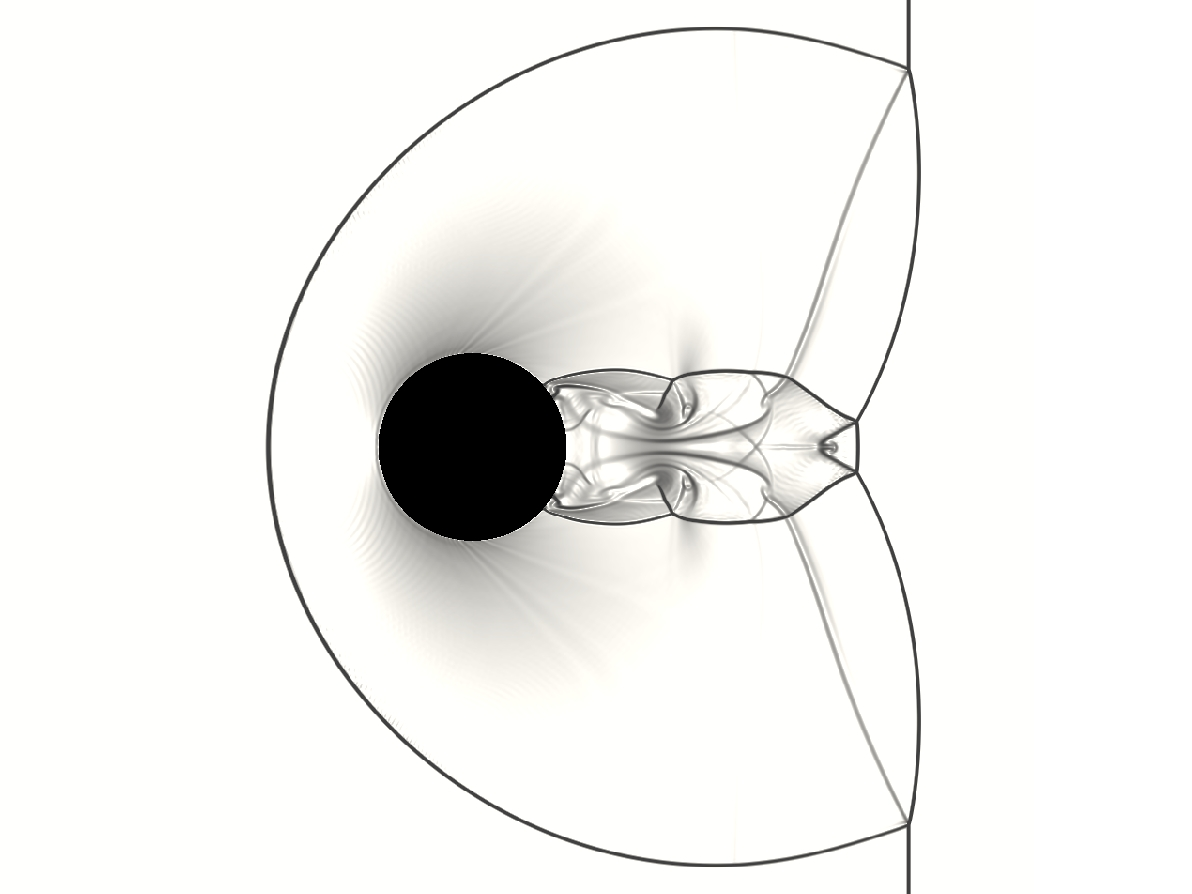
\includegraphics[trim = 30mm 0mm 30mm 0mm, clip, width=0.40\textwidth]{shock_cyn}
    \bicaption{激波圆柱作用。}{Shock-cylinder interaction.}
    \label{fig:shock_cyn}
\end{figure}

多图的插入如图\ref{fig:oaspl},多图不应在子图中给文本子标题,只要给序号,并在主标题中进行引用说明。
\begin{figure}[!htbp]
    \centering
    \begin{subfigure}[b]{0.35\textwidth}
      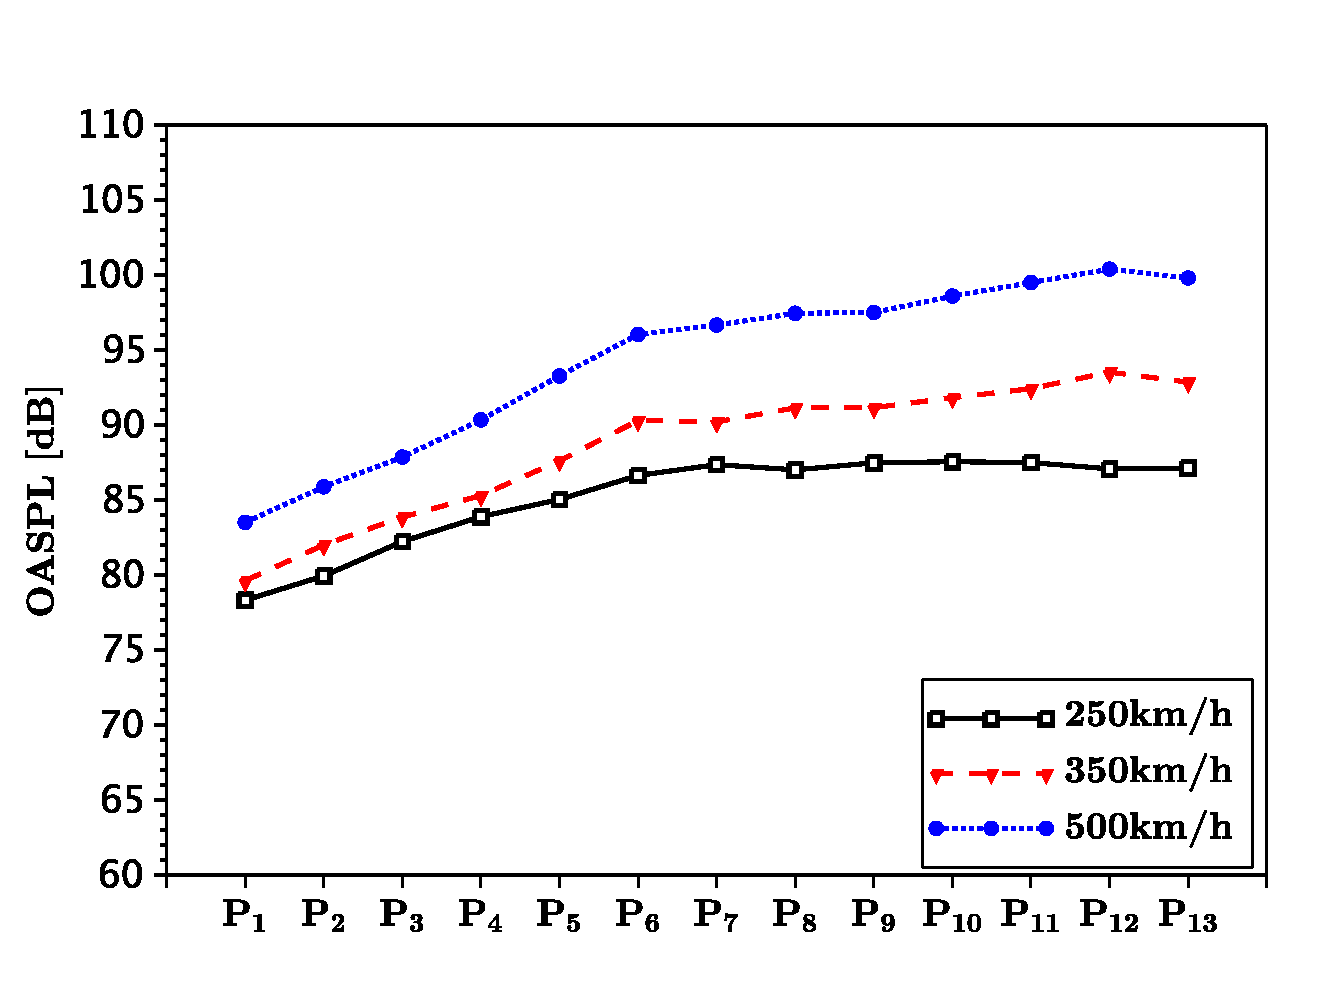
\includegraphics[width=\textwidth]{oaspl_a}
      \caption{}
      \label{fig:oaspl_a}
    \end{subfigure}%
    ~% add desired spacing
    \begin{subfigure}[b]{0.35\textwidth}
      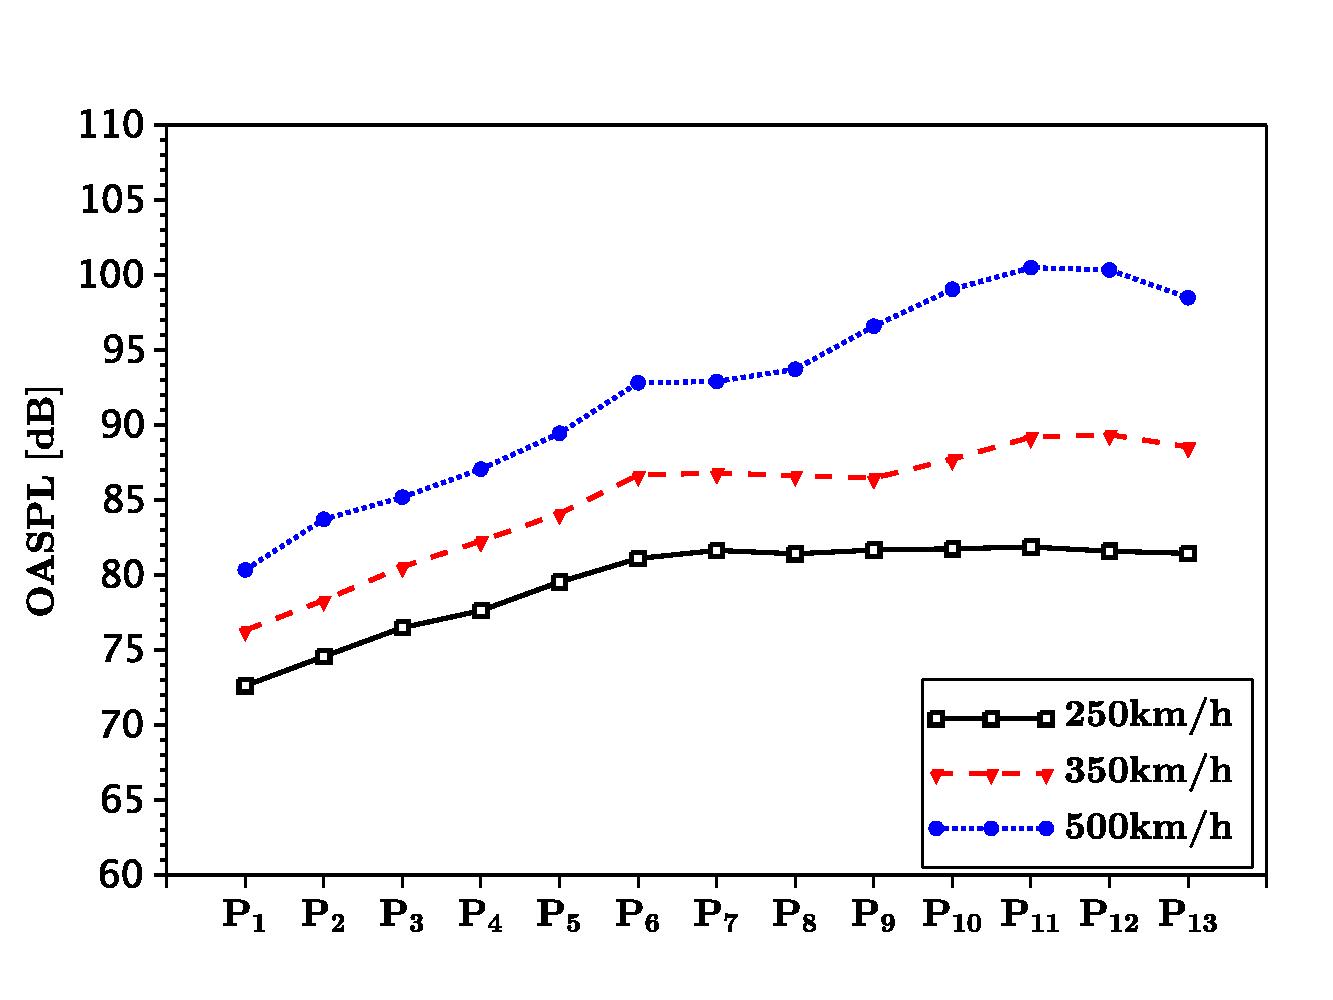
\includegraphics[width=\textwidth]{oaspl_b}
      \caption{}
      \label{fig:oaspl_b}
    \end{subfigure}
    \\% line break
    \begin{subfigure}[b]{0.35\textwidth}
      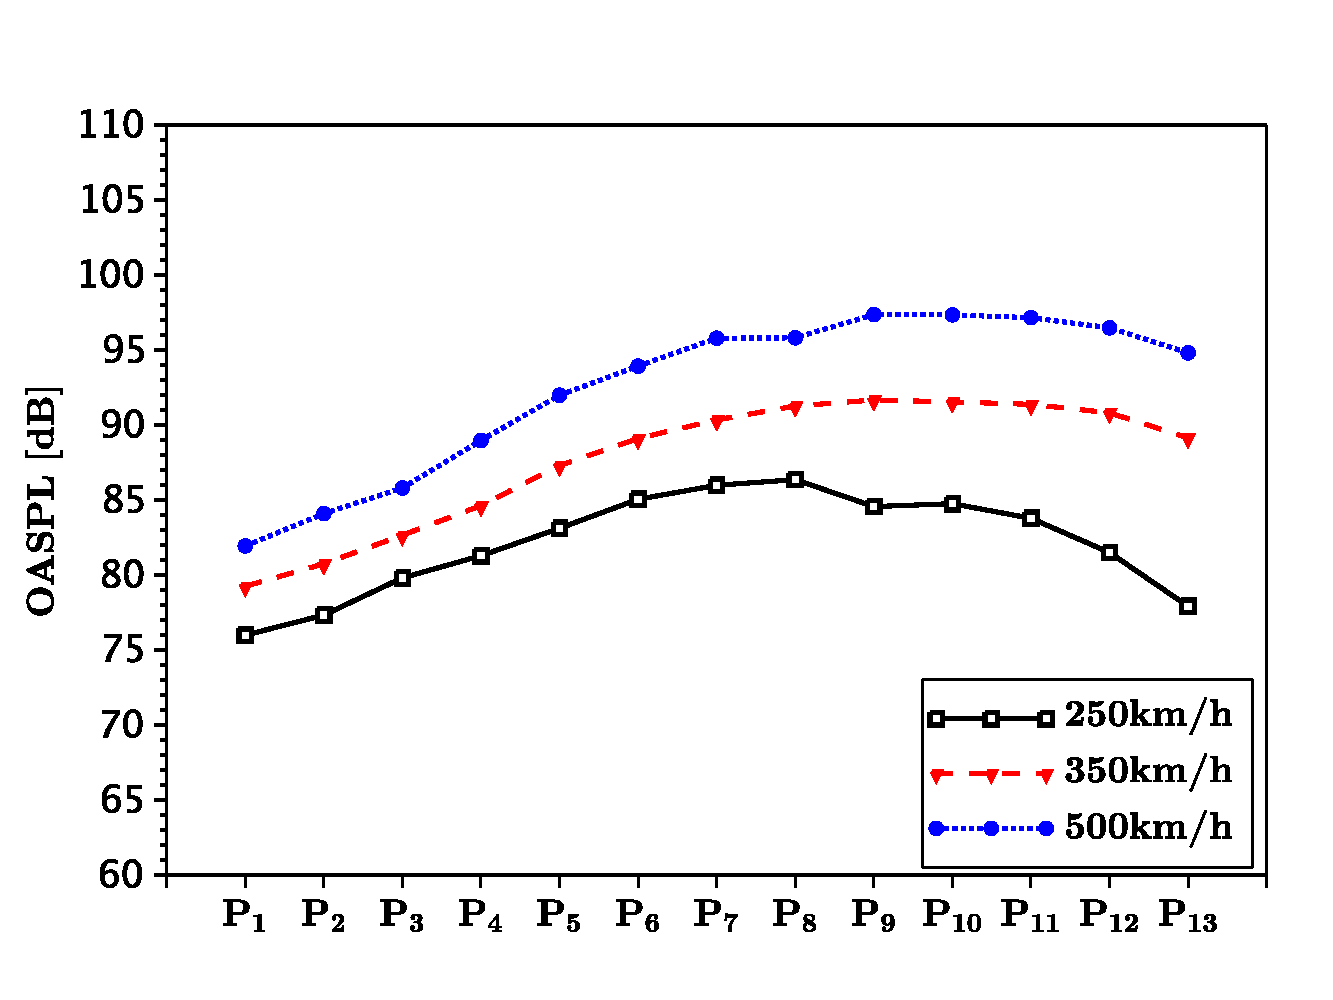
\includegraphics[width=\textwidth]{oaspl_c}
      \caption{}
      \label{fig:oaspl_c}
    \end{subfigure}%
    ~% add desired spacing
    \begin{subfigure}[b]{0.35\textwidth}
      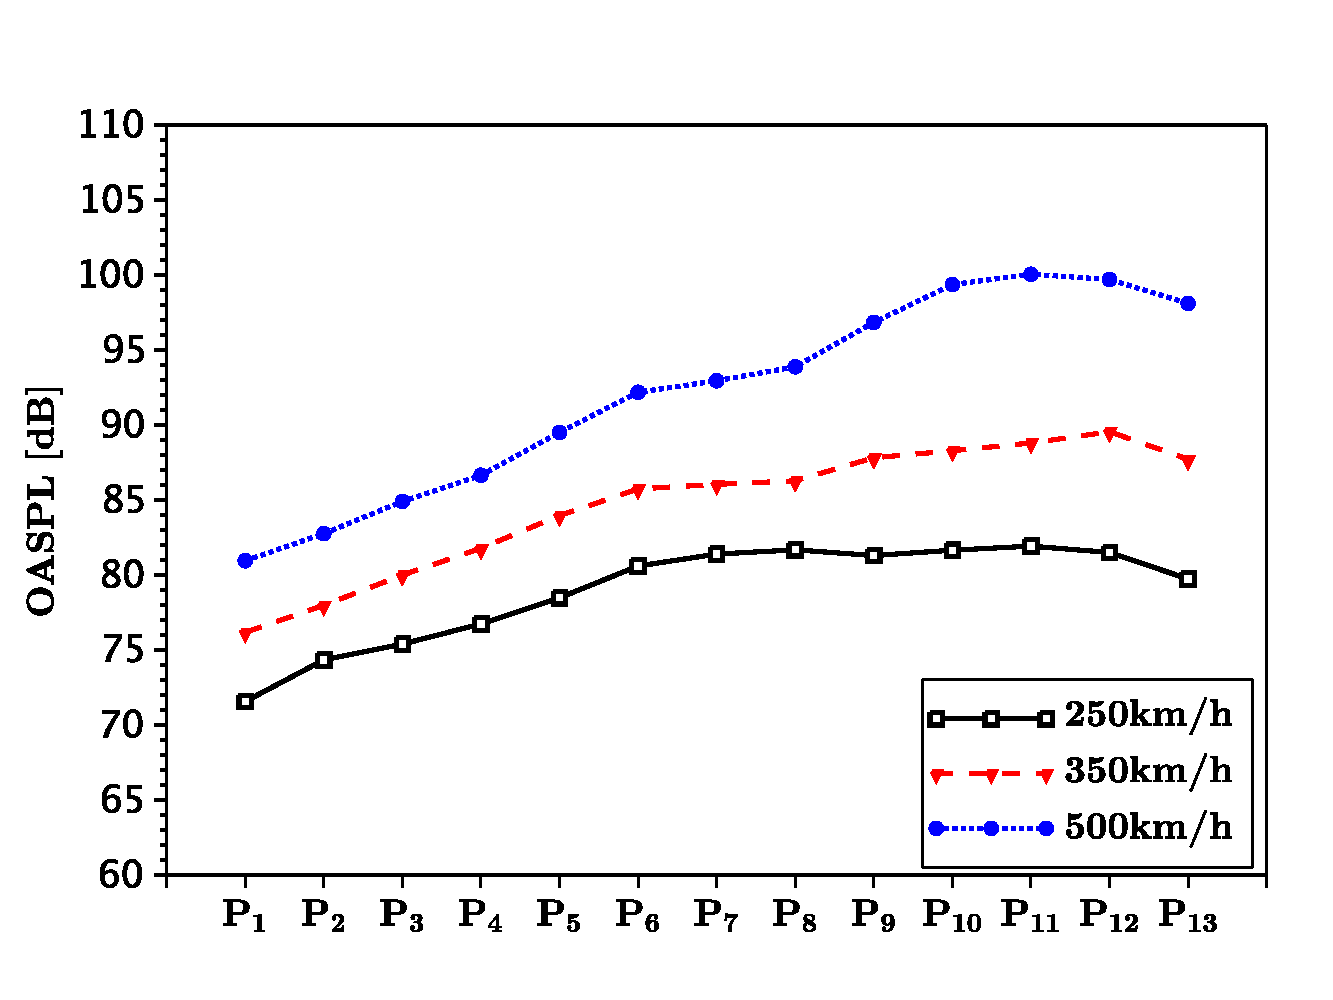
\includegraphics[width=\textwidth]{oaspl_d}
      \caption{}
      \label{fig:oaspl_d}
    \end{subfigure}
    \bicaption{总声压级。(a) 这是子图说明信息,(b) 这是子图说明信息,(c) 这是子图说明信息,(d) 这是子图说明信息。}{OASPL.(a) This is the explanation of subfig, (b) This is the explanation of subfig, (c) This is the explanation of subfig, (d) This is the explanation of subfig.}
    \label{fig:oaspl}
\end{figure}

\subsection{算法}

如见算法~\ref{alg:euclid},详细使用方法请参见文档 \href{https://ctan.org/pkg/algorithmicx?lang=en}{algorithmicx}。

\begin{algorithm}[!htbp]
    \small
    \caption{Euclid's algorithm}\label{alg:euclid}
    \begin{algorithmic}[1]
        \Procedure{Euclid}{$a,b$}\Comment{The g.c.d. of a and b}
        \State $r\gets a\bmod b$
        \While{$r\not=0$}\Comment{We have the answer if r is 0}
        \State $a\gets b$
        \State $b\gets r$
        \State $r\gets a\bmod b$
        \EndWhile\label{euclidendwhile}
        \State \textbf{return} $b$\Comment{The gcd is b}
        \EndProcedure
    \end{algorithmic}
\end{algorithm}

\subsection{参考文献引用}

参考文献引用过程以实例进行介绍,假设需要引用名为"Document Preparation System"的文献,步骤如下:

1)使用Google Scholar搜索Document Preparation System,在目标条目下点击Cite,展开后选择Import into BibTeX打开此文章的BibTeX索引信息,将它们copy添加到ref.bib文件中(此文件位于Biblio文件夹下)。

2)索引第一行 \verb|@article{lamport1986document,|中 \verb|lamport1986document| 即为此文献的label (\textbf{中文文献也必须使用英文label},一般遵照:姓氏拼音+年份+标题第一字拼音的格式),想要在论文中索引此文献,有两种索引类型:

文本类型:\verb|\citet{lamport1986document}|。正如此处所示 \citet{lamport1986document}; 

括号类型:\verb|\citep{lamport1986document}|。正如此处所示 \citep{lamport1986document}。

\textbf{多文献索引用英文逗号隔开}:

\verb|\citep{lamport1986document, chu2004tushu, chen2005zhulu}|。正如此处所示 \citep{lamport1986document, chu2004tushu, chen2005zhulu}

更多例子如:

\citet{walls2013drought} 根据 \citet{betts2005aging} 的研究,首次提出...。其中关于... \citep{walls2013drought, betts2005aging},是当前中国...得到迅速发展的研究领域 \citep{chen1980zhongguo, bravo1990comparative}。引用同一著者在同一年份出版的多篇文献时,在出版年份之后用
英文小写字母区别,如:\citep{yuan2012lana, yuan2012lanb, yuan2012lanc} 和 \citet{yuan2012lana, yuan2012lanb, yuan2012lanc}。同一处引用多篇文献时,按出版年份由近及远依次标注。例如 \citep{chen1980zhongguo, stamerjohanns2009mathml, hls2012jinji, niu2013zonghe}。

使用著者-出版年制(authoryear)式参考文献样式时,中文文献必须在BibTeX索引信息的 \textbf{key} 域(请参考ref.bib文件)填写作者姓名的拼音,才能使得文献列表按照拼音排序。参考文献表中的条目(不排序号),先按语种分类排列,语种顺 序是:中文、日文、英文、俄文、其他文种。然后,中文按汉语拼音字母顺序排列,日文按第一著者的姓氏笔画排序,西文和 俄文按第一著者姓氏首字母顺序排列。如中 \citep{niu2013zonghe}、日 \citep{Bohan1928}、英 \citep{stamerjohanns2009mathml}、俄 \citep{Dubrovin1906}。

如此,即完成了文献的索引,请查看下本文档的参考文献一章,看看是不是就是这么简单呢?是的,就是这么简单!

不同文献样式和引用样式,如著者-出版年制(authoryear)、顺序编码制(numbers)、上标顺序编码制(super)可在Thesis.tex中对artratex.sty调用实现,详见 \href{https://github.com/mohuangrui/ucasthesis/wiki}{ucasthesis 知识小站之文献样式}

%若在上标顺序编码制(super)模式下,希望在特定位置将上标改为嵌入式标,可使用 \citetns{niu2013zonghe,stamerjohanns2009mathml} 和 \citepns{niu2013zonghe,stamerjohanns2009mathml}。

参考文献索引的更多知识,请见 \href{https://en.wikibooks.org/wiki/LaTeX/Bibliography_Management}{WiKibook Bibliography}。\nocite{*}% 使文献列表显示所有参考文献(包括未引用文献)

\section{常见使用问题}\label{sec:qa}

\begin{enumerate}
    \item 模板每次发布前,都已在Windows,Linux,MacOS系统上测试通过。下载模板后,若编译出现错误,则请见 \href{https://github.com/mohuangrui/ucasthesis/wiki}{ucasthesis知识小站} 的 \href{https://github.com/mohuangrui/ucasthesis/wiki/%E7%BC%96%E8%AF%91%E6%8C%87%E5%8D%97}{编译指南}。

    \item 模板文档的编码为UTF-8编码。所有文件都必须采用UTF-8编码,否则编译后生成的文档将出现乱码文本。若出现文本编辑器无法打开文档或打开文档乱码的问题,请检查编辑器对UTF-8编码的支持。如果使用WinEdt作为文本编辑器(\textbf{不推荐使用}),应在其Options -> Preferences -> wrapping选项卡下将两种Wrapping Modes中的内容:
        
        TeX;HTML;ANSI;ASCII|DTX...
        
        修改为:TeX;\textbf{UTF-8|ACP;}HTML;ANSI;ASCII|DTX...
        
        同时,取消Options -> Preferences -> Unicode中的Enable ANSI Format。

    \item 推荐选择xelatex或lualatex编译引擎编译中文文档。编译脚本的默认设定为xelatex编译引擎。你也可以选择不使用脚本编译,如直接使用 \LaTeX{}文本编辑器编译。注:\LaTeX{}文本编辑器编译的默认设定为pdflatex编译引擎,若选择xelatex或lualatex编译引擎,请进入下拉菜单选择。为正确生成引用链接和参考文献,需要进行\textbf{全编译}。

    \item Texmaker使用简介
        \begin{enumerate}
            \footnotesize
            \item 使用 Texmaker “打开 (Open)” Thesis.tex。
            \item 菜单 “选项 (Options)” -> “设置当前文档为主文档 (Define as Master Document)”
            \item 菜单 “自定义 (User)” -> “自定义命令 (User Commands)” -> “编辑自定义命令 (Edit User Commands)” -> 左侧选择 “command 1”,右侧 “菜单项 (Menu Item)” 填入 Auto Build -> 点击下方“向导 (Wizard)” -> “添加 (Add)”: xelatex + bibtex + xelatex + xelatex + pdf viewer -> 点击“完成 (OK)”
            \item 使用 Auto Build 编译带有未生成引用链接的源文件,可以仅使用 xelatex 编译带有已经正确生成引用链接的源文件。
            \item 编译完成,“查看(View)” PDF,在PDF中 “ctrl+click” 可链接到相对应的源文件。
        \end{enumerate}
    
    \item 模版的设计可能地考虑了适应性。致谢等所有条目都是通过最为通用的

        \verb+\chapter{item name}+  and \verb+\section*{item name}+

        来显式实现的 (请观察Backmatter.tex),从而可以随意添加,放置,和修改,如同一般章节。对于图表目录名称则可在ucasthesis.cfg中进行修改。

    \item 设置文档样式: 在artratex.sty中搜索关键字定位相应命令,然后修改
        \begin{enumerate}
            \item 正文行距:启用和设置 \verb|\linespread{1.5}|,默认1.5倍行距。
            \item 参考文献行距:修改 \verb|\setlength{\bibsep}{0.0ex}|
            \item 目录显示级数:修改 \verb|\setcounter{tocdepth}{2}|
            \item 文档超链接的颜色及其显示:修改 \verb|\hypersetup|
        \end{enumerate}

    \item 文档内字体切换方法:
        \begin{itemize}
            \item 宋体:国科大论文模板ucasthesis 或 \textrm{国科大论文模板ucasthesis}
            \item 粗宋体:{\bfseries 国科大论文模板ucasthesis} 或 \textbf{国科大论文模板ucasthesis}
            \item 黑体:{\sffamily 国科大论文模板ucasthesis} 或 \textsf{国科大论文模板ucasthesis}
            \item 粗黑体:{\bfseries\sffamily 国科大论文模板ucasthesis} 或 \textsf{\bfseries 国科大论文模板ucasthesis}
            \item 仿宋:{\ttfamily 国科大论文模板ucasthesis} 或 \texttt{国科大论文模板ucasthesis}
            \item 粗仿宋:{\bfseries\ttfamily 国科大论文模板ucasthesis} 或 \texttt{\bfseries 国科大论文模板ucasthesis}
            \item 楷体:{\itshape 国科大论文模板ucasthesis} 或 \textit{国科大论文模板ucasthesis}
            \item 粗楷体:{\bfseries\itshape 国科大论文模板ucasthesis} 或 \textit{\bfseries 国科大论文模板ucasthesis}
        \end{itemize}
\end{enumerate}


